%Please use LuaLaTeX or XeLaTeX
\documentclass[11pt,aspectratio=169,reqno]{beamer}

\title{Math meets Biology}
\date[28.03.2023]{28.03.2023}
\author{Mario Kunz, Xaver Hanushevsky}
\institute{D-BIOL}

\usetheme{eth}

\colorlet{titlefgcolor}{ETHBlue}
\colorlet{accentcolor}{ETHRed}

\begin{document}

\titleframe

\begin{frame}[fragile]{Intro}
    Etwas Kreatives einfallen lassen für hier
\end{frame}

\begin{frame}{Rückkopplung}
\end{frame}

\begin{frame}{Repression des lac-operons}
Zeichnung des Schemas, vorerst aber ohne Beachtung der Bindung von Lactose/Allolactose
\end{frame}

\begin{frame}{Genregulation über DNA-bindendes Protein}
    \begin{figure}
        \centering
        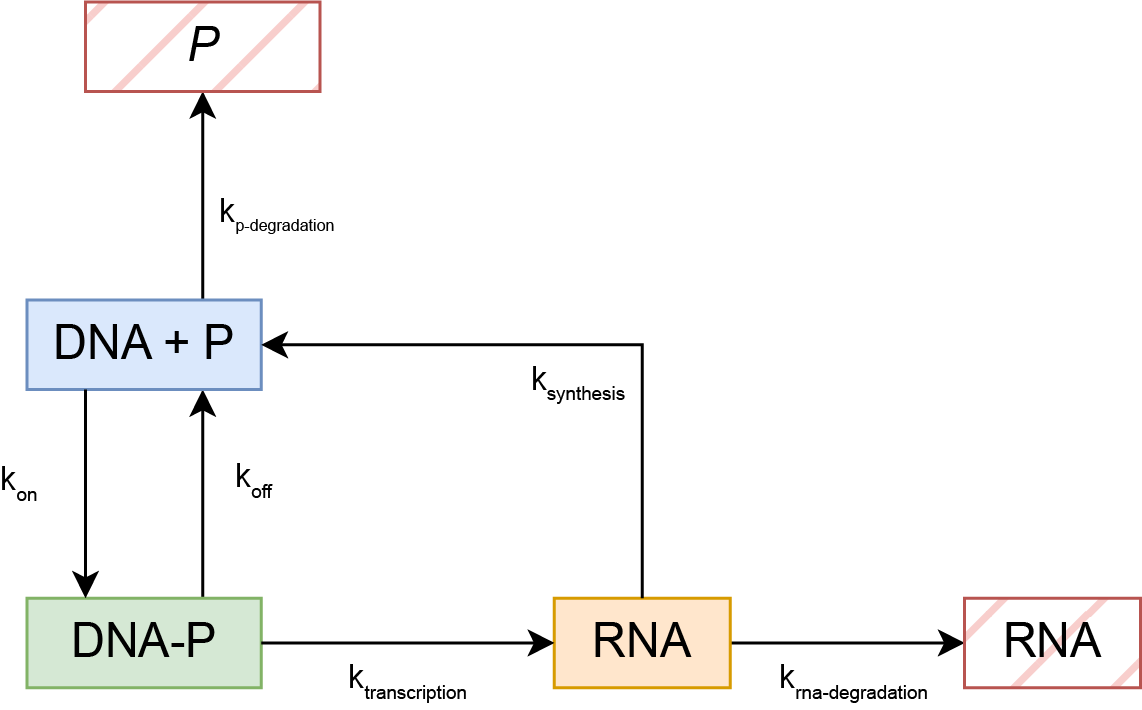
\includegraphics[width=.6\textwidth]{images/Schema Genregulation Regulation.png}
        \label{fig:my_label}
    \end{figure}
\end{frame}

\begin{frame}{Gleichgewicht zwischen gebundener und freier DNA}
Herleitung für den Ausdruck der Konzentration der gebundenen DNA $[D]$
\end{frame}

\begin{frame}{Vergleich mit Glockshuber}
\end{frame}

\begin{frame}{Mathematische Modellierung}
\begin{equation}
    \frac{d[\text{RNA}]}{dt}=[\text{RNA}]_{\text{Synthese}}-[\text{RNA}]_{\text{Abbau}}
\end{equation}
\\[12pt]
\begin{equation}
    \frac{d[P]}{dt}=[P]_{\text{Synthese}}-[P]_{\text{Abbau}}
\end{equation}
\end{frame}

\begin{frame}[t]{Mathematische Modellierung mRNA}
    \begin{tabular}{l l}
        $\dfrac{d[\text{RNA}]}{dt} =[\text{RNA}]_{\text{Synthese}}-\textcolor{red}{[\text{RNA}]_{\text{Abbau}}}$ &  \\
    \end{tabular}
    \begin{equation}\notag
        [\text{RNA}]_{\text{Abbau}}=[\text{RNA}] \cdot k_{dr}
    \end{equation}
\end{frame}

\begin{frame}[t]{Mathematische Modellierung mRNA}
w2    \begin{tabular}{l l}
        $\dfrac{d[\text{RNA}]}{dt} =[\text{RNA}]_{\text{Synthese}}-{[\text{RNA}]_{\text{Abbau}}}$ &  \\
    \end{tabular}
    \begin{equation}\notag
        [\text{RNA}]_{\text{Abbau}}=[\text{RNA}] \cdot k_{dr}
    \end{equation}
    \\[16pt]
    \begin{tabular}{l l}
        $\dfrac{d[\text{RNA}]}{dt} =\textcolor{red}{[\text{RNA}]_{\text{Synthese}}}-{[\text{RNA}]_{\text{Abbau}}}$ &  \\
    \end{tabular}
    \begin{equation}\notag
        [\text{RNA}]_{\text{Synthese}}=v_{\text{max}}\cdot\frac{K}{K+[P]}
    \end{equation}
\end{frame}

\begin{frame}[t]{Mathematische Modellierung mRNA}
    \begin{tabular}{l l}
        $\dfrac{d[\text{RNA}]}{dt} =[\text{RNA}]_{\text{Synthese}}-\textcolor{ETHBlue}{[\text{RNA}]_{\text{Abbau}}}$ &  \\
    \end{tabular}
    \begin{equation}\notag
        \textcolor{ETHBlue}{
        [\text{RNA}]_{\text{Abbau}}}=[\text{RNA}] \cdot k_{dr}
    \end{equation}
    \\[16pt]
    \begin{tabular}{l l}
        $\dfrac{d[\text{RNA}]}{dt} =\textcolor{ETHPurple}{[\text{RNA}]_{\text{Synthese}}}-[\text{RNA}]_{\text{Abbau}}$ &  \\
    \end{tabular}
    \begin{equation}\notag
    \textcolor{ETHPurple}{[\text{RNA}]_{\text{Synthese}}}=v_{\text{max}}\cdot\frac{K}{K+[P]}
    \end{equation}
    \\[16pt]
    \begin{equation}\tag{1}
        \frac{d[\text{RNA}]}{dt}=v_{\text{max}}\cdot\frac{K}{K+[P]}-[\text{RNA}] \cdot k_{dr}
    \end{equation}
\end{frame}

\begin{frame}[t]{Mathematische Modellierung Protein}
    \begin{tabular}{l l}
        $\dfrac{d[P]}{dt} =[P]_{\text{Synthese}}-{[P]_{\text{Abbau}}}$ &  \\
    \end{tabular}
    \begin{equation}\notag
        [P]_{\text{Abbau}}=[P] \cdot k_{dr}
    \end{equation}
    \\[16pt]
    \begin{equation}\notag
        [P]_{\text{Synthese}}=k_{s}\cdot[\text{RNA}]
    \end{equation}
    \\[16pt]
    \begin{equation}\tag{2}
        \frac{d[P]}{dt}=k_{s}\cdot[\text{RNA}]-[P] \cdot k_{dr}
    \end{equation}
\end{frame}

\begin{frame}{Mathematische Modellierung}

\begin{align}
    \frac{d[\text{RNA}]}{dt}&=v_{\text{max}}\cdot\frac{K}{K+[P]}-[\text{RNA}] \cdot k_{dr} \tag{1} \\[16pt]
    \frac{d[P]}{dt}&=k_{s}\cdot[\text{RNA}]-[P] \cdot k_{dr} \tag{2}
\end{align}

\end{frame}

\begin{frame}{Stationäre Lösung mRNA}\end{frame}

\begin{frame}{Stationäre Lösung Protein}
Nur eines der beiden herleiten
\end{frame}

\begin{frame}{Numerische Lösung mit Matlab}
\end{frame}

\begin{frame}{Biologische Bedeutung}
\end{frame}

\begin{frame}{Vergleich mit positiver Rückkopplung}
\end{frame}

\end{document}